
%TODO: aggiungere roba da pagine 0 a pagina 109
%WARN: arrivato al paragrafo "circlo di Deming(PDCA)" pag 155

\chapter{Ingegneria dei processi aziendali}


\section{Azienda}
\subsection{Visione per funzioni Vs per processi}

I processi vengono svolti da risorse umane presenti nelle
divisioni aziendali o funzioni(dipartimenti aziendale
specifico per funzione).

Alcune definizioni di funzione aziendale:
\begin{quote}
	\textit{
		Le funzioni sono aggregazioni di uomini e
		mezzi necessari per lo svolgimento di
		attività della stessa natura
	}
	D. Pierantozzi
\end{quote}

\begin{quote}
	\textit{
		In un’impresa organizzata per funzioni le
		attività simili, che assolvono cioè la
		stessa funzione, che richiedono le
		stesse competenze e che utilizzano lo
		stesso tipo di risorse e di tecnologie,
		vengono raggruppate	in	un’unità	organizzativa
		sotto	un’unica	responsabilità
	}
	E. Bartezzaghi
\end{quote}


L'intera azienda viene divisa in \textbf{unità organizzative funzionali},
ciascuna delle quali può essere suddivisa in reparti, uffici, ecc.


Mentre le \textbf{funzioni} ragruppano attività \textbf{simili},
le \textbf{attività} ragruppano anche attività di \textbf{diversa}
naturali ma che \textbf{collaborano} per raggiungere un obiettivo comune.



\subsection{Business Peocess Management(BPM)}
Il BPM è una metodologia utilizzata dalle organizzazioni per migliorare continuamente
i processi di business operativi(interni ed interorganizzativi).

Il BPM si può riassumere in 4 passi:
\begin{enumerate}
	\item Definire e mappare il processo di business
	\item Identificare i modi per migliroare le fasi del processo che aggiungono valore
	\item Identificare modi per eliminare fasi che non aggiungono valore
	\item Adattare i workflow informatici per riflettere i cambiamenti
\end{enumerate}


\subsubsection{Workflow Vs Business Process}

La definizione di workflow è la seguente:
\begin{quote}
	\textit{
		An automation of a business process, in whole or
		part, during which documents, information or tasks are passed
		from one participant to another for action, according to a set
		of procedural rules.
	}
\end{quote}

Mentre la definizione di business process è la seguente:
\begin{quote}
	\textit{
		A set of one or more linked procedures or
		activities which collectively realize a business objective or
		policy goal, normally within the context of an organizational
		structure defining functional roles and relationships.
	}
\end{quote}

Quindi un \textbf{processo aziendale} è qualsiasi attività che realizza obiettivi aziendali,
mentre \textbf{workflow} è un'automazione(parziale) di un processo aziendale.


\begin{figure}[!ht]
	\centering
	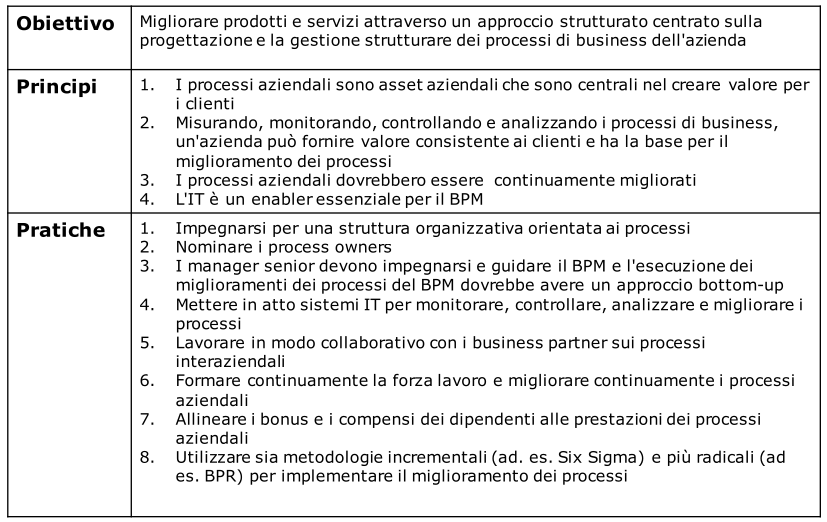
\includegraphics[width=0.7\textwidth]{./images/bpm_principi_pratiche.png}
	\caption{BPM: principi e pratiche}
	\label{fig:bpm_principi_pratiche}
\end{figure}


\subsubsection{Principi del BPM}
\begin{enumerate}
	\item Difendere cultura del processo
	\item Attivare catene interne di clienti e fornitori
	\item Bilanciare logiche pull e push
	\item Decentrare processi e gestione informazioni
	\item Usare ICT(Information and Communication Technology) per ridisegnare i processi
	\item Ricomporre attività frammiste
	\item Introdurre delega decisionale
	\item Realizzare orgnizzazioni snella e flessibili(Lean Office)
\end{enumerate}

\subsubsection{Six Sigma e Lean Office}

Il \textbf{Six Sigma} nasce in ambito produzione di \textit{Motorola} e si concentra
su minimizzare difetti con la misurazione dell'output dei processi.


Il \textbf{Lean Office} nasce in ambito produzione di \textit{Toyota} e si concentra
sull'eliminazione di sprechi(attività che non portano valore al cliente), il BPM
pone enfasi su IT(Information Technology) come strumento per migliorare i processi di business.



\subsection{Nuove tecnologie per BP}

\begin{itemize}
  \item \textbf{Process Mining}: è una tecnica di analisi dei log dei sistemi informativi
  \item \textbf{Robotic Process Automation}: utilizzo di bot per esecuzioni automatiche
  \item \textbf{Intelligent BPMS}: Componenti di BPM che utilizzano AI per migliorare i processi
\end{itemize}




\subsection{Variabili organizzative}
Le 4 variabili organizzative sono:
\begin{enumerate}
  \item \textbf{Organizzazione del processo}: mediante organigramma, tabelle delle proprietà, LRC(Linear Responsibility Chart) o RACI
  \item \textbf{Flusso delle attività}: sequenze di attività, attività, attori, eventi, oggetti
  \item \textbf{Competenze delle risorse umame}: competenze, formazione, figure professionali
  \item \textbf{Misurazione e controllo delle prestazioni}: pianificazione e controllo dei costi e del valore per il cliente, KPI(Key Performance Indicator)
\end{enumerate}



\section{Il Ciclo di Deming(PDCA)}

